\documentclass[resume]{subfiles}


\begin{document}
\section{Wireless}
$$\boxed{\lambda=\frac{c}{f}}$$
\section{Transmission sans-fil}
$$\SI{1}{\watt}=\SI{30}{\deci\bel m}$$
\subsection{Formule de Friis}
Dans un cas idéal, sans trajets multiples
$$\frac{P_r}{P_t}=G_tG_r\left(\frac{\lambda}{4\pi R}\right)^2$$
en \si{\deci\bel} : 
$$\underbrace{(P_r)_{\si{\deci\bel}}-(P_t)_{\si{\deci\bel}}}_{-Att_{\si{\deci\bel}}}=(G_t)_{\si{\deci\bel}}+(G_r)_{\si{\deci\bel}}+20\log_{10}\left(\frac{\lambda}{4\pi R}\right)$$
$$A_{tt_{\si{\deci\bel}}}>0$$
$$(x)_{\si{\deci\bel}}=10\log_{10}(x)$$
A noter que la puissance de 2 a été enlevée et le $10\log$ remplacé par $20\log$
\subsubsection{Avec $\gamma$}
$$\frac{P_r}{P_t}=G_tG_r\left(\frac{\lambda}{4\pi}\right)^2\frac{1}{R^\gamma}$$
\begin{multline*}
\underbrace{(P_r)_{\si{\deci\bel}}-(P_t)_{\si{\deci\bel}}}_{-Att_{\si{\deci\bel}}}=(G_t)_{\si{\deci\bel}}+(G_r)_{\si{\deci\bel}}+\\20\log_{10}\left(\frac{\lambda}{4\pi}\right)+10\log_{10}\left(\frac{1}{R^{\gamma}}\right)
\end{multline*}
\paragraph{Valeurs de $\gamma$} Espace libre 2, Environnement urbain 2.7 à 3.5, environnement urbain avec ombrage 3 à 5, dans un bâtiment avec vue de l'antenne 1.6 à 1.8, dans un bâtiment sans vue 4 à 6, dans une industrie 2 à 3

Si on rajoute $\gamma$ après-coup, on utilise la formule suivante pour calculer la nouvelle atténuation $\text{Att}_\gamma$ (on considère $\text{Att}>0$) :
$$\text{Att}_\gamma = \text{Att}+10\log_{10}(r^{\gamma-2})$$
\subsection{zone de Fresnel}
\begin{figure}[H]
\centering
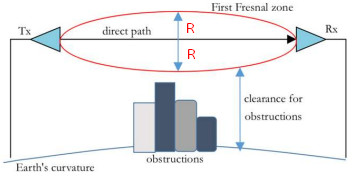
\includegraphics[width=0.5\columnwidth]{img_0.png}
\end{figure}
$$R=\frac{1}{2}\sqrt{\frac{cD}{f}}$$
Avec $D$ la distance entre les antennes, $c$ la vitesse de la lumière et $f$ la fréquence

\end{document}